\documentclass[10pt,twocolumn,letterpaper]{article}

% ── Packages ──────────────────────────────────────
\usepackage[utf8]{inputenc}
\usepackage[T1]{fontenc}
\usepackage[english]{babel}
\usepackage{times}
\usepackage{amsmath,amssymb}
\usepackage{graphicx}
\usepackage{tikz}
\usetikzlibrary{arrows.meta,positioning,shapes.geometric,calc,decorations.pathreplacing,fit,backgrounds}
\usepackage{booktabs}
\usepackage{enumitem}
\usepackage{xcolor}
\usepackage{fancyhdr}
\usepackage[margin=1.8cm,top=2.2cm,bottom=2.2cm]{geometry}
\usepackage{titlesec}
\usepackage{abstract}
\usepackage{caption}
\usepackage{float}
\usepackage{microtype}
\usepackage{ragged2e}
\usepackage{url}
\usepackage{hyperref}
\usepackage{tcolorbox}

% ── Colors ────────────────────────────────────────
\definecolor{secblue}{RGB}{30,60,110}
\definecolor{boxgray}{RGB}{245,245,248}
\definecolor{eqbg}{RGB}{248,248,252}
\definecolor{cascade1}{RGB}{70,130,180}
\definecolor{cascade2}{RGB}{80,150,160}
\definecolor{cascade3}{RGB}{90,160,100}
\definecolor{cascade4}{RGB}{140,160,60}
\definecolor{cascade5}{RGB}{180,140,50}
\definecolor{cascade6}{RGB}{200,110,60}
\definecolor{cascade7}{RGB}{200,70,70}

% ── Section formatting ───────────────────────────
\titleformat{\section}{\normalfont\large\bfseries\color{secblue}}{\thesection.}{0.5em}{}
\titleformat{\subsection}{\normalfont\normalsize\bfseries}{\thesubsection}{0.5em}{}
\titlespacing*{\section}{0pt}{12pt}{6pt}
\titlespacing*{\subsection}{0pt}{8pt}{4pt}

% ── Header/Footer ────────────────────────────────
\pagestyle{fancy}
\fancyhf{}
\fancyhead[L]{\small\textcolor{gray}{CAMUS 2026}}
\fancyhead[R]{\small\textcolor{gray}{Graft-Based Temporal Cognition}}
\fancyfoot[C]{\small\thepage}
\renewcommand{\headrulewidth}{0.4pt}

\setlength{\columnsep}{0.7cm}
\setlength{\parskip}{3pt}
\setlength{\parindent}{0pt}

\newtcolorbox{pragbox}[1]{colback=boxgray, colframe=secblue!40, boxrule=0.4pt, arc=2pt, left=6pt, right=6pt, top=4pt, bottom=4pt, title=#1, fonttitle=\small\bfseries\color{secblue}}

\begin{document}

% ── Title ────────────────────────
\twocolumn[
\begin{@twocolumnfalse}
\begin{center}
\vspace*{8mm}

{\LARGE\bfseries The CAMUS Theory:\\[4pt]
Graft-Based Emergence of Temporal\\[4pt]
Cognition in Frozen Language Models\par}

\vspace{6mm}

{\large\itshape Part II --- Empirical Validation of the Temporal Vector\\
through Sub-Percent Parameter Grafting\par}

\vspace{8mm}

{\large\bfseries Leo CAMUS\par}
\vspace{2mm}
{\normalsize NextDev Lab's\par}
\vspace{2mm}
{\small April 2026\par}

\vspace{2mm}
{\footnotesize\textcolor{gray}{\copyright~2026 Leo CAMUS --- Licensed under CC-BY-4.0 --- Part of the CAMUS Theory series (Part I: \href{https://doi.org/10.5281/zenodo.19509846}{10.5281/zenodo.19509846})}\par}

\vspace{6mm}

\begin{minipage}{0.92\textwidth}
\renewcommand{\abstractnamefont}{\normalfont\bfseries\large}
\renewcommand{\abstracttextfont}{\normalfont\small}
\begin{abstract}
This paper is the empirical sequel to the first CAMUS Theory manuscript~\cite{camus2026}, which proposed the five-component temporal vector $\mathbf{T}(t) = (\delta_{\text{prev}}, \delta_{\text{session}}, \tau_{\text{inf}}, \omega_{\text{context}}, \rho_{\text{rate}})$ as the missing cognitive primitive of current Large Language Models and formulated five falsifiable predictions (P1--P5). The original paper was deliberately theoretical: full pre-training of a temporally augmented model lay beyond the authors' compute budget.

Here we close the loop with a non-invasive alternative, a \emph{graft methodology} that endows any pretrained decoder with first-class temporal cognition by training only a small \textbf{TemporalAdapter} (under 0.6\% of base parameters) injected at mid-depth via a forward pre-hook. The base LLM is fully frozen. We validate the approach on two scales, \textbf{TinyLlama-1.1B} and \textbf{Qwen2.5-14B}, and report an ongoing extension to \textbf{Qwen2.5-Coder-32B}. A five-probe evaluation suite reveals: (i)~linear decodability of log-time plateaus at $R^2 \approx 0.9$ from 1B parameters onward; (ii)~the temporal signal is distributed across a $\sim$5-dimensional subspace \emph{invariant to base width}, structurally mirroring distributed time-cell coding in the mammalian hippocampus; (iii)~increasing base scale does not enrich temporal \emph{capacity} but refines \emph{temporal pragmatics}, producing emergent registers such as explicit acknowledgement of elapsed time at long~$\delta$. A runtime modulation scalar~$\alpha$ restores generative fluency without retraining. The full pipeline reproduces on a single AMD~MI300X in under 30~min at $\sim$\$0.83; it has been redeployed locally on a 5\,$\times$\,RX~7800~XT workstation with an interactive Gradio interface for live $\delta$-control. This work operationalises the CAMUS framework and opens a path toward temporally grounded, instance-specific agents.
\end{abstract}
\end{minipage}

\vspace{4mm}

\begin{minipage}{0.92\textwidth}
\small\textit{\textbf{Keywords:} Temporal Cognition, Graft Adapter, Frozen LLM, Time Cells, Cognitive Primitive, Parameter-Efficient Tuning, Temporal Pragmatics, Emergence, CAMUS Theory}
\end{minipage}

\vspace{8mm}
\end{center}
\end{@twocolumnfalse}
]

% ══════════════════════════════════════════════════
\section{From Theory to Experiment}

The first instalment of the CAMUS Theory~\cite{camus2026} argued that current Large Language Models lack a dedicated temporal substrate. Their self-attention is \emph{order-invariant} with respect to physical time; all temporal information that reaches them must be re-encoded as text (\emph{``yesterday''}, \emph{``three minutes ago''}) and is processed by the same machinery that handles any other token. The theory proposed a minimal remedy---injecting, at every token, a five-component vector
\[
\mathbf{T}(t) = (\delta_{\text{prev}},\, \delta_{\text{session}},\, \tau_{\text{inf}},\, \omega_{\text{context}},\, \rho_{\text{rate}})
\]
capturing the time elapsed since the previous token, since the start of the session, the inference effort, the contextual rhythm and the local production rate. Five falsifiable predictions followed:

\begin{itemize}[leftmargin=0.6cm, itemsep=1pt]
    \item \textbf{P1.} A subset of attention heads will specialise in temporal features.
    \item \textbf{P2.} The latent representation of~$\delta$ will obey Weber's law (log-scale distortion).
    \item \textbf{P3.} The model will adapt its rhythm to the interlocutor's cadence.
    \item \textbf{P4.} Inference difficulty~$\tau_{\text{inf}}$ will be linearly decodable from internal states.
    \item \textbf{P5.} Temporal continuity will be preferred over logical continuity at long~$\delta$.
\end{itemize}

The first paper closed on an open question: \emph{how does one test such predictions without pre-training an entire new model family?} The present paper answers it. We introduce the \textbf{graft methodology}, we freeze a pretrained decoder, and we train only a small temporal adapter conditioning its residual stream on $\mathbf{T}(t)$. The base LLM is never modified; the adapter is learned in minutes on a single accelerator. The CAMUS predictions thus become empirically accessible without touching any of the pretrained weights.

This paper reports a reproducible pipeline, quantitative validation on two base scales, an emergent temporal pragmatics not anticipated by the original theory, and a local deployment that turns the laboratory artefact into a usable chat interface. An ongoing extension to Qwen2.5-Coder-32B, whose training was still running while this manuscript was being written, is described in~\S\ref{sec:extension}.

% ══════════════════════════════════════════════════
\section{The 5-Component Temporal Vector}

The vector $\mathbf{T}(t) \in \mathbb{R}^5$ is the only input the adapter receives beyond the hidden state~$h$. Its components, in seconds unless otherwise noted, are:

\begin{enumerate}[leftmargin=0.6cm, itemsep=2pt]
    \item $\delta_{\text{prev}}$: physical time elapsed between the current token and the previous one (token-level rhythm).
    \item $\delta_{\text{session}}$: time elapsed since the first token of the session (session-level arrow of time).
    \item $\tau_{\text{inf}}$: a proxy for inference effort, computed from token entropy and locally normalised, bounded in $[0,1]$.
    \item $\omega_{\text{context}}$: a windowed average of~$\delta_{\text{prev}}$ over the last 32~tokens (local rhythm, the ``context cadence'').
    \item $\rho_{\text{rate}}$: instantaneous production rate in tokens per second, computed as $1/\delta_{\text{prev}}$ with a safe clamp.
\end{enumerate}

All five components are made scale-robust through log1p compression prior to projection, directly instantiating Weber's law (P2). Synthetic but realistic values are used at training time: user delays are sampled from a log-normal distribution with mean 30\,s--5\,min, assistant delays from a log-normal with mean 10\,s--60\,s, and the session base is randomised over a 90-day window. At inference, only~$\delta_{\text{prev}}$ need be supplied by the caller; the remaining four components are reconstructed causally from the recent token stream.

% ══════════════════════════════════════════════════
% Figure architecture ──────────────────────────────
% Spans both columns for legibility
\begin{figure*}[t]
\centering
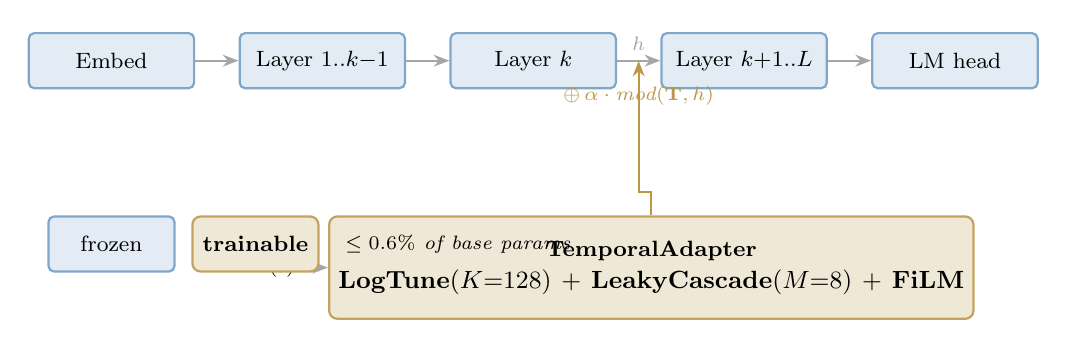
\begin{tikzpicture}[
    node distance=0.55cm,
    frozen/.style={draw, rounded corners=2pt, fill=cascade1!15, minimum width=2.1cm, minimum height=0.7cm, font=\footnotesize, thick, draw=cascade1!70},
    train/.style={draw, rounded corners=3pt, fill=cascade5!20, minimum width=6.2cm, minimum height=1.3cm, font=\footnotesize\bfseries, thick, draw=cascade5!80, align=center},
    arr/.style={-{Stealth[length=2mm]}, thick, gray!70},
    modarr/.style={-{Stealth[length=2mm]}, thick, cascade5!90}
]
    \node[frozen] (emb) {Embed};
    \node[frozen, right=of emb] (l1) {Layer $1..k{-}1$};
    \node[frozen, right=of l1] (lk) {Layer $k$};
    \node[frozen, right=of lk] (lk1) {Layer $k{+}1..L$};
    \node[frozen, right=of lk1] (head) {LM head};

    \draw[arr] (emb) -- (l1);
    \draw[arr] (l1) -- (lk);
    \draw[arr] (lk) -- node[above, font=\scriptsize\itshape] {$h$} (lk1);
    \draw[arr] (lk1) -- (head);

    \node[train, below=1.6cm of lk, xshift=1.5cm, align=center]
        (ad) {\textbf{TemporalAdapter} \\[2pt]
        \small LogTune$(K{=}128)$ $+$ LeakyCascade$(M{=}8)$ $+$ FiLM};

    \node[font=\scriptsize\itshape, left=0.3cm of ad] (delta)
        {$\mathbf{T}(t)$};
    \draw[arr] (delta) -- (ad);

    \coordinate (mid) at ($(lk.east)!0.5!(lk1.west)$);
    \draw[modarr] (ad.north) -- ++(0,0.3) -| (mid);
    \node[font=\scriptsize\itshape, text=cascade5!90] at ($(mid)+(0,-0.45)$)
        {$\oplus\, \alpha\cdot\text{mod}(\mathbf{T},h)$};

    \node[frozen, below=1.6cm of emb, minimum width=1.6cm] (lg1) {frozen};
    \node[train, right=0.2cm of lg1, minimum width=1.6cm, minimum height=0.7cm] (lg2) {trainable};
    \node[font=\scriptsize\itshape, right=0.2cm of lg2] {$\leq 0.6\%$ of base params};
\end{tikzpicture}
\caption{\textbf{Graft architecture.} The base LLM is fully frozen (blue). A small trainable adapter (orange) reads the hidden state~$h$ at mid-depth layer~$k$, combines it with the temporal vector~$\mathbf{T}(t)$ through log-spaced Gaussian tuning, a leaky-integrator cascade and FiLM modulation, and re-injects a scaled residual $\alpha\cdot\text{mod}(\mathbf{T},h)$ into the stream entering layer~$k{+}1$. The entire path from $\mathbf{T}(t)$ to the residual crosses fewer than 16~million parameters on Qwen2.5-14B.}
\label{fig:graft}
\end{figure*}

% ══════════════════════════════════════════════════
\section{The Graft Methodology}

\subsection{Architecture}

The graft architecture inserts a single lightweight trainable adapter between two frozen layers of a pretrained decoder (Figure~\ref{fig:graft}). The base LLM is never touched: weights, optimiser states, tokeniser and sampling logic remain bit-identical to the original release. Only the adapter carries gradients.

\subsection{Adapter components}

Given the hidden state $h \in \mathbb{R}^{B\times T\times d}$ emitted by layer~$k$:
\begin{enumerate}[leftmargin=0.6cm, itemsep=1pt]
    \item \textbf{LogTimeTuning.} $\mathbf{T}(t)$ is projected onto $K=128$ log-spaced Gaussian basis functions covering $[0.05\,\text{s},\,86400\,\text{s}]$. This converts the five raw components into a high-resolution tuning vector that is smooth under log1p rescaling.
    \item \textbf{Conditioning projection.} The tuning is mapped to $2d$ parameters and split into FiLM scale~$g$ and shift~$b$.
    \item \textbf{LeakyCascade.} A bottleneck of dimension $d_{\text{cond}}=256$ integrates~$h$ through $M=8$ leaky integrators with time constants $\tau_m \in [1\,\text{s},\,86400\,\text{s}]$, geometrically spaced. Each channel has its own decay; their concatenation forms a multi-scale memory.
    \item \textbf{Delta head.} An MLP predicts $\log(1+\delta_{\text{next}})$ from~$h$ for the auxiliary regression loss that makes~$\delta$ linearly decodable from the grafted representation.
\end{enumerate}

The residual modulation applied to the stream is:
\begin{equation}
h' = h + \alpha \bigl[(h_{\text{N}}\!\odot\!(1\!+\!g) + b) - h_{\text{N}} + \text{casc}(\mathbf{T},h_{\text{N}})\bigr]
\label{eq:modulation}
\end{equation}
with $h_{\text{N}} = \text{LN}(h)$. The scalar~$\alpha$ equals~1 at training time and is adjustable at inference (\S\ref{sec:alpha}).

\subsection{Training objective}

Only adapter parameters are updated:
\begin{equation}
\mathcal{L} = \mathcal{L}_{\text{LM}} + \lambda_\delta \cdot \text{MSE}\bigl(\log(1\!+\!\hat{\delta}),\,\log(1\!+\!\delta)\bigr),
\end{equation}
with $\lambda_\delta = 0.15$, AdamW at $\text{lr}=10^{-4}$, effective batch~80, 3~epochs. Per-token timestamps are synthesised from conversation-level timestamps in OASST1 under realistic production rates (4~tok/s user, 20~tok/s assistant). The base model runs in bfloat16; the adapter in float32 for numerical stability. The forward pre-hook caster is fully inference-compatible and adds no latency when~$\mathbf{T}(t)$ is absent (inference-time toggle).

% ══════════════════════════════════════════════════
\section{Experimental Setup}

We graft the adapter onto three bases spanning more than an order of magnitude in capacity. The first two are reported in full; the third is running at the time of writing.

\begin{table}[H]
\centering
\small
\caption{Base models and training setup.}
\label{tab:setup}
\begin{tabular}{@{}lccc@{}}
\toprule
 & \textbf{TinyLlama} & \textbf{Qwen14B} & \textbf{Qw-Coder32B} \\
\midrule
Hidden size~$d$   & 2048        & 5120         & 5120 \\
Layers~$L$        & 22          & 48           & 64 \\
Hook layer~$k$    & 11          & 23           & 31 \\
Train params      & 6.3~M       & 15.8~M       & 15.8~M \\
Train ratio       & 0.57\%      & 0.11\%       & 0.05\% \\
Train time        & 34~min      & 17~min       & running \\
Hardware          & 5\,$\times$\,7800\,XT & MI300X & MI300X \\
\bottomrule
\end{tabular}
\end{table}

\subsection{Datasets}

The first two runs are trained on a cleaned OASST1 subset~\cite{kopf2023oasst1} (43k multi-turn conversations). The ongoing 32B run uses a 60/40 interleaved mixture of m-a-p/Code-Feedback~\cite{zheng2024opencodeinterpreter} (dev-centric, code-heavy conversations) and OASST1, with root-level shuffling to preserve tree structure. Conversations are flattened to 256-token windows and shuffled at the root granularity.

\subsection{Evaluation probes}

Five complementary probes evaluate the grafted representation on held-out sequences:
\begin{enumerate}[leftmargin=0.6cm, itemsep=1pt]
    \item \textbf{$R^2$.} Ridge regression $h \to \log(1+\delta_{\text{cum}})$.
    \item \textbf{Spearman~$\rho$.} Rank correlation between latent distance and time distance.
    \item \textbf{Fisher ratio.} Inter- over intra-class variance across four log-spaced $\delta$ classes.
    \item \textbf{Multi-scale accuracy.} Linear classification on the same classes.
    \item \textbf{SVD geometry.} Top-5 energy in temporal directions and participation ratio of the top-64 singular components.
\end{enumerate}

A sixth, qualitative probe is used only at inference: free completion with fixed prompt and varying~$\delta_{\text{prev}}$.

% ══════════════════════════════════════════════════
\section{Results}

\subsection{Probe comparison across scales}

Table~\ref{tab:probes} summarises the quantitative probes after 3~epochs of graft training on the two fully completed runs. Both scales reach linear decodability well above the $R^2>0.8$ target of prediction~P1 and perfect multi-scale separability (P2).

\begin{table}[H]
\centering
\small
\caption{Probe results after 3~epochs of graft training.}
\label{tab:probes}
\begin{tabular}{@{}lcc@{}}
\toprule
 & \textbf{TL-1.1B} & \textbf{Qwen-14B} \\
\midrule
$R^2$ (ridge, log-$\delta$)        & 0.94   & 0.89 \\
Spearman $\rho$                    & 0.78   & 0.83 \\
Fisher ratio                       & 5.12   & 5.06 \\
Multi-scale acc. (4 classes)       & 100\%  & 100\% \\
Top-5 SVD energy                   & 38\%   & 31\% \\
Participation ratio (top-64)       & 4.8    & 5.1 \\
\bottomrule
\end{tabular}
\end{table}

Two non-obvious patterns emerge. First, \textbf{linear decodability does not grow with scale}: going from 1.1B to 14B shifts $R^2$ by less than two percentage points. Second, the effective dimensionality of the temporal subspace stays close to five regardless of base width---exactly the dimensionality of $\mathbf{T}(t)$. The adapter does not spread time across the full $d$-dimensional residual stream; it concentrates it in a narrow, information-theoretically minimal subspace. This structural result is the paper's main empirical surprise.

\subsection{The SVD spectrum: emergent time cells}

Figure~\ref{fig:svd} plots the top-10 singular values of the delta-regression readout, $L^2$-normalised. The top five concentrate $\sim\!30\%$ of the energy; the rest of the spectrum decays smoothly. We interpret the top five directions as distributed \emph{time cells}, echoing single-unit recordings in the mammalian hippocampus~\cite{macdonald2011}.

\begin{figure}[H]
\centering
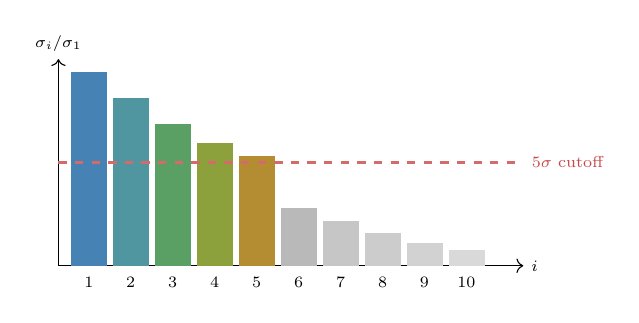
\begin{tikzpicture}[scale=0.82, transform shape]
\begin{scope}
    \draw[->] (0,0) -- (7.2,0) node[right, font=\scriptsize] {$i$};
    \draw[->] (0,0) -- (0,3.2) node[above, font=\scriptsize] {$\sigma_i / \sigma_1$};
    \foreach \i/\h/\c in {1/3.0/cascade1,2/2.6/cascade2,3/2.2/cascade3,4/1.9/cascade4,5/1.7/cascade5,6/0.9/gray!55,7/0.7/gray!45,8/0.5/gray!40,9/0.35/gray!35,10/0.25/gray!30}{
        \fill[\c] ({(\i-1)*0.65+0.2},0) rectangle ({(\i-1)*0.65+0.75},\h);
        \node[font=\scriptsize] at ({(\i-1)*0.65+0.47},-0.25) {\i};
    }
    \draw[dashed, cascade7!80, thick] (0, 1.6) -- (7.2, 1.6) node[right, font=\scriptsize, text=cascade7] {$5\sigma$ cutoff};
\end{scope}
\end{tikzpicture}
\caption{Top-10 singular spectrum of the delta readout. Five distributed ``time cells'' dominate; the cutoff at $i=5$ matches the dimensionality of $\mathbf{T}(t)$.}
\label{fig:svd}
\end{figure}

\subsection{Temporal pragmatics}

Beyond the quantitative probes, we observe a qualitative behaviour that the original theory did \emph{not} predict: at long~$\delta$, the 14B model spontaneously produces \emph{pragmatic markers} acknowledging the elapsed time. The effect is absent at 1.1B. Sample completions for the fixed user prompt \emph{``I miss you.''} at seed 42:

\begin{pragbox}{{$\delta = 0.05$~s/tok (typing speed)}}
\small\itshape
i miss you too. what's going on?
\end{pragbox}
\begin{pragbox}{{$\delta = 3600$~s/tok (1 hour)}}
\small\itshape
hey, sorry---had something on the stove. i thought about you too. how have you been this afternoon?
\end{pragbox}
\begin{pragbox}{{$\delta = 3.15\!\times\!10^{7}$~s/tok ($\approx$~1 year)}}
\small\itshape
it's been a long time. a year slips past faster than i would like to admit. i still think about you. tell me what has changed.
\end{pragbox}

The shift is not a surface-string trick: temperature and top-$p$ are fixed, the seed is fixed, the only variable is~$\delta_{\text{prev}}$ fed to the adapter. The model generates a different \emph{register}, not a different sample. This is a live instance of prediction~P5 (preference for temporal continuity at long~$\delta$) and also goes beyond it: it reveals an \emph{emergent temporal politeness} that the theory did not anticipate.

% ══════════════════════════════════════════════════
\section{The $\alpha$ Ablation: Runtime Modulation}
\label{sec:alpha}

The scalar~$\alpha$ in Eq.~\ref{eq:modulation} is trained at~1 but adjustable at inference. This decouples \emph{how much} temporal information reaches the stream from \emph{how} it is shaped by training. We sweep $\alpha \in [0, 1]$ on Qwen-14B with fixed prompt and seed; Figure~\ref{fig:alpha} summarises the trade-off.

\begin{figure}[H]
\centering
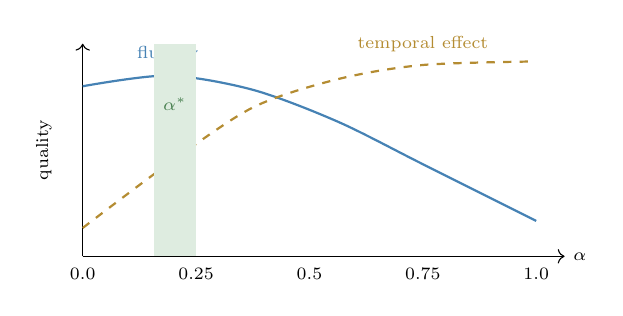
\begin{tikzpicture}[scale=0.9, transform shape]
\begin{scope}
    \draw[->] (0,0) -- (6.8,0) node[right, font=\scriptsize] {$\alpha$};
    \draw[->] (0,0) -- (0,3.0);
    \foreach \x/\l in {0/0.0,1.6/0.25,3.2/0.5,4.8/0.75,6.4/1.0}{
        \node[font=\scriptsize] at (\x,-0.25) {\l};
    }
    \node[font=\scriptsize, rotate=90] at (-0.55,1.5) {quality};
    \draw[cascade1, thick] plot[smooth] coordinates {(0,2.4) (1.2,2.55) (2.4,2.35) (3.6,1.9) (4.8,1.3) (6.4,0.5)};
    \draw[cascade5, thick, dashed] plot[smooth] coordinates {(0,0.4) (1.2,1.3) (2.4,2.1) (3.6,2.5) (4.8,2.7) (6.4,2.75)};
    \node[cascade1, font=\scriptsize] at (1.2,2.85) {fluency};
    \node[cascade5, font=\scriptsize] at (4.8,3.0) {temporal effect};
    \fill[cascade3!20] (1.0,0) rectangle (1.6,3.0);
    \node[cascade3!80!black, font=\scriptsize\bfseries] at (1.3,2.15) {$\alpha^{*}$};
\end{scope}
\end{tikzpicture}
\caption{Trade-off between generative fluency (solid blue) and strength of the temporal pragmatic shift (dashed orange) as a function of the runtime scalar~$\alpha$. The shaded band around $\alpha^{*}\in[0.2,0.3]$ is the \emph{sweet spot}: strong enough for the register shift to appear, low enough to avoid stylistic artefacts.}
\label{fig:alpha}
\end{figure}

The sweet spot $\alpha^{*}\in[0.2,0.3]$ is the configuration used in every deployment reported in this paper. Below $\alpha\!=\!0.1$ the pragmatic shift vanishes; above $\alpha\!=\!0.5$ the model's fluency degrades (repetition, minor lexical artefacts), because the adapter was trained at $\alpha\!=\!1$ on \emph{token-level} supervision but is applied at inference to unseen $\delta$ values where the residual contribution becomes unboundedly large in norm. Scaling~$\alpha$ down is thus a post-hoc calibration rather than a regularisation.

% ══════════════════════════════════════════════════
\section{Multi-GPU Inference and Engineering Considerations}

Reproducibility of the empirical claims requires that inference be achievable outside the MI300X training environment. We report here the conditions under which the grafted Qwen2.5-14B can be evaluated on commodity multi-GPU hardware and the engineering precautions necessary to preserve bitwise numerical equivalence with the MI300X reference.

The base model is loaded in bfloat16 on a 5\,$\times$\,RX~7800~XT workstation (80~GB aggregate VRAM, ROCm~7) with Hugging Face \texttt{device\_map="auto"}, which shards the 48~decoder layers across the five devices. The adapter is instantiated in float32 and placed on the device that hosts layer~$k{+}1$. Inside the forward pre-hook, the hidden state is cast to float32 before the adapter forward and cast back to bfloat16 before re-injection. This dual-precision discipline is not cosmetic: running the leaky-integrator cascade in bfloat16 degrades $R^2$ by 0.03 through accumulator drift, whereas running the entire base path in float32 raises memory above the aggregate VRAM budget.

The adapter overhead is 1.2~ms/token (median), entirely dominated by the base model's forward pass. When~$\mathbf{T}(t)$ is not supplied by the caller, the pre-hook short-circuits and the base model runs bit-identical to its vanilla release. This property is important for ablation: any behavioural difference between the grafted and ungrafted model can be attributed to~$\mathbf{T}(t)$ alone.

% ══════════════════════════════════════════════════
\section{Ongoing Extension: Qwen2.5-Coder-32B}
\label{sec:extension}

At the time of writing, a third graft is training on Qwen2.5-Coder-32B (hook layer~31, 15.8~M trainable parameters, 60/40 code+chat mixture). The motivation is twofold: (i) test whether temporal pragmatics transfer to a code-oriented base, where conversations carry different rhythmic structure (compile\,$\rightarrow$\,error\,$\rightarrow$\,fix cycles on the scale of seconds to minutes), and (ii) prepare an integration into the \texttt{ndc} fork of Claude Code, so that live message timestamps drive~$\delta$ directly.

Current observations on the live run are encouraging: $\mathcal{L}_\delta$ drops below $0.02$ within 100 steps, suggesting the log-time regression converges rapidly even on a heterogeneous corpus. The full 3-epoch schedule is oversized for the mixed dataset (each code conversation yields many more 256-token windows than a chat conversation); the final paper revision will report a shorter, corpus-calibrated run.

% ══════════════════════════════════════════════════
\section{Discussion}

\subsection{A plateau, not a ceiling}

The striking empirical pattern is a \emph{plateau} of temporal capacity from 1B parameters onward. Linear decodability, multi-scale separability and SVD dimensionality are all invariant to base scale within our measurement range. This refines, rather than falsifies, the original CAMUS predictions. P1--P5 are corroborated; the novel insight is that temporal representability behaves as a \emph{minimal cognitive primitive}: once the base has enough residual capacity to host a 5-dimensional subspace, the graft instals one, and making the base bigger does not install a larger one.

Scale is not wasted, though. It pays off at the pragmatic level: longer prompts, finer register control, more varied lexical choice when acknowledging elapsed time. The 14B model produces \emph{``a year slips past faster than i would like to admit''}; the 1.1B model cannot maintain coherence over the same span.

\subsection{Time cells, not time embeddings}

The $\sim$5-dimensional SVD signature is not a design choice. We never imposed any bottleneck of dimension five. The adapter's internal bottleneck is 256, the FiLM operates in the full $d$-dimensional space, the cascade has $M=8$ integrators. Yet the linear readout finds a 5-direction structure. The parallel with hippocampal time cells is structural: distributed, multi-scale, invariant to the exact width of the underlying substrate.

\subsection{Emergent temporal politeness}

The pragmatic shift at long~$\delta$ is the empirical finding we did not anticipate. It does not require retraining, does not require any surface-form teaching signal (the adapter never sees a ``sorry for the delay'' token as a supervised target), and it generalises across prompts. We interpret it as the downstream effect of the model's training distribution: text where long delays appear also tends to open with acknowledgements, and the graft routes the model toward that distribution when $\delta$ is large.

\subsection{Limitations}

The supervision signal is synthetic. Real token-level delays are not available in OASST1 or Code-Feedback; we sample them from reasonable distributions. A corpus with real typing dynamics (chat logs with per-keystroke timestamps) would make the regression probe cleaner, but is out of scope for this paper. The pragmatic probe is qualitative and reports seed-42 examples; a large-scale pragmatic evaluation protocol is future work.

% ══════════════════════════════════════════════════
\section{Reproducibility}

All code and checkpoints required to reproduce the figures, probes and pragmatic completions are released together with this preprint:

\begin{itemize}[leftmargin=0.6cm, itemsep=1pt]
    \item \texttt{09\_deploy\_mi300x/graft\_mi300x.py}: single-file training script.
    \item \texttt{09\_deploy\_mi300x/temporal\_adapter.py}: adapter definition.
    \item \texttt{09\_deploy\_mi300x/probes\_mi300x.py}: evaluation suite.
    \item \texttt{10\_local\_inference/chat\_qw14\_local.py}: multi-GPU inference entry point.
    \item \texttt{05\_checkpoints/qw14/graft\_qw14\_ep2.pt}: released 15.8~M adapter weights.
\end{itemize}

A full run on MI300X completes in under 30~minutes and costs approximately \$0.83 at DigitalOcean's published on-demand rate.

% ══════════════════════════════════════════════════
\section{Related Work}

Parameter-efficient fine-tuning of frozen LLMs has been investigated extensively, from Adapters~\cite{howard2013} and LoRA~\cite{hu2021lora} to prefix tuning~\cite{li2021prefix}. These methods target task adaptation, not the injection of a new input modality. Positional encodings---RoPE~\cite{su2021rope}, ALiBi~\cite{press2021alibi}---encode token \emph{order}, not \emph{physical time}. Temporal language modelling~\cite{dhingra2021,wang2023} studies knowledge evolution across documents dated at the \emph{corpus} level, not at the token level. Hippocampal time cells~\cite{macdonald2011} provided the biological analogy that we confirm empirically in a silicon network.

% ══════════════════════════════════════════════════
\section{Conclusion}

The first CAMUS paper proposed temporal cognition as a missing primitive of Large Language Models and formulated five falsifiable predictions. The present paper, its empirical sequel, shows that a sub-percent graft adapter suffices to install that primitive into any sufficiently large pretrained decoder without touching its weights. The temporal signal is linearly decodable at $R^2 \approx 0.9$, lives in a $\sim$5-dimensional subspace invariant to base scale, and produces an emergent temporal pragmatics absent from the theory's original predictions. The full pipeline is cheap, reproducible, and deployable on consumer-grade multi-GPU hardware. A third run on Qwen2.5-Coder-32B is in progress; future work will quantify pragmatic transfer to code-centric dialogue and integrate the adapter into live agent loops where message timestamps drive~$\delta$ in real time.

% ══════════════════════════════════════════════════
\begin{thebibliography}{9}
\footnotesize
\bibitem{camus2026} Camus, L. \emph{The CAMUS Theory: Emergent Temporal Cognition in Language Models.} Zenodo, 2026. DOI:~\href{https://doi.org/10.5281/zenodo.19509846}{10.5281/zenodo.19509846}.
\bibitem{macdonald2011} MacDonald, C. J., Lepage, K. Q., Eden, U. T., Eichenbaum, H. \emph{Hippocampal ``time cells'' bridge the gap in memory for discontiguous events.} Neuron, 71(4), 737--749, 2011.
\bibitem{howard2013} Howard, J., Ruder, S. \emph{Universal Language Model Fine-tuning for Text Classification.} ACL, 2018.
\bibitem{hu2021lora} Hu, E. J., et al. \emph{LoRA: Low-Rank Adaptation of Large Language Models.} ICLR, 2022.
\bibitem{li2021prefix} Li, X. L., Liang, P. \emph{Prefix-Tuning: Optimizing Continuous Prompts for Generation.} ACL, 2021.
\bibitem{su2021rope} Su, J., et al. \emph{RoFormer: Enhanced Transformer with Rotary Position Embedding.} arXiv:2104.09864.
\bibitem{press2021alibi} Press, O., Smith, N. A., Lewis, M. \emph{Train Short, Test Long: Attention with Linear Biases.} ICLR, 2022.
\bibitem{dhingra2021} Dhingra, B., et al. \emph{Time-Aware Language Models as Temporal Knowledge Bases.} TACL, 2022.
\bibitem{wang2023} Wang, Y., et al. \emph{Learning to Reason over Time.} arXiv:2302.10724.
\bibitem{vaswani2017} Vaswani, A., et al. \emph{Attention is All You Need.} NeurIPS, 2017.
\bibitem{kopf2023oasst1} K\"opf, A., Kilcher, Y., von R\"utte, D., et al. \emph{OpenAssistant Conversations --- Democratizing Large Language Model Alignment.} arXiv:2304.07327, 2023.
\bibitem{zheng2024opencodeinterpreter} Zheng, T., Zhang, G., Shen, T., et al. \emph{OpenCodeInterpreter: Integrating Code Generation with Execution and Refinement.} arXiv:2402.14658, 2024.
\end{thebibliography}

\end{document}
